\documentclass[addpoints]{exam}

\usepackage[top=2cm, bottom=2cm, left=2cm, right=2cm]{geometry}
\usepackage[utf8]{inputenc}
\usepackage[icelandic]{babel}
\usepackage[T1]{fontenc}
\usepackage[sc]{mathpazo}

\makeatletter % Fix due to (recent versions of?) minted containing their own framed definition
\expandafter\providecommand\expandafter*\csname ver@framed.sty\endcsname
{2003/07/21 v0.8a Simulated by exam}
\makeatother

\usepackage{minted} 
\usepackage[parfill]{parskip}
\usepackage{booktabs,tabularx}
\usepackage{multirow}
\usepackage{multicol}
\usepackage{graphicx}
\usepackage{enumerate}
\usepackage{amsmath, amsfonts, amssymb, amsthm}

\usepackage[bookmarks=true,colorlinks=true,pdfauthor={Eirikur Ernir Thorsteinsson},linkcolor=blue,urlcolor=blue]{hyperref}

\setcounter{secnumdepth}{-1} 
\hyphenpenalty=5000

\newcommand\blankpage{%
    \null
    \thispagestyle{empty}%
    \addtocounter{page}{-1}%
    }

\usemintedstyle{default}
\renewcommand{\theFancyVerbLine}{\sffamily \arabic{FancyVerbLine}}
\author{}
\date{}

\footer{}{}{}

\qformat{\large \textbf Spurning \thequestion \phantom{M}(\totalpoints \phantom{l}stig) \hfill}
\renewcommand{\solutiontitle}{\noindent\textbf{Svar:}\par\noindent}
\renewcommand{\points}{stig}
\renewcommand{\questionshook}{\setlength{\itemsep}{0.5cm}}
\hqword{Spurning:}
\hpword{Stig í boði:}
\hsword{Stig:}
\htword{Samtals}

\newmintedfile[cppfile]{cpp}{frame=lines, linenos=false}
\newmintedfile[javafile]{java}{frame=lines, linenos=false}
\newcommand{\eng}[1]{(e.\ \emph{#1})}

\title{TÖL203G Tölvunarfræði 2 - upptökupróf}
\author{}
\date{7. júní 2017}

\pagestyle{headandfoot}
\firstpageheader{TÖL203G \\ Tölvunarfræði 2}{Upptökupróf}{7. júní 2017}
\firstpagefooter{}{Bls. \thepage\ af \numpages}{}
\runningfooter{}{Bls. \thepage\ af \numpages}{}
\setlength{\columnsep}{0.5cm}

% \printanswers
\begin{document}

% \thispagestyle{empty}
Fullt nafn: \vspace*{1mm} \hrule

\begin{center}
\begin{minipage}{.8\textwidth}

\vspace{5cm}

\textbf{Leiðbeiningar:} Á þessu prófi eru \numquestions\ spurningar sem samtals gefa \numpoints\ stig. 
Skrifið svör beint á þessar síður. 
Ef meira pláss vantar, skrifið á bakhlið viðkomandi síðu. 
Leyfileg hjálpargögn eru reiknivél og ein A4 blaðsíða af glósum. 
Dæmi prófsins eru misþung og eru ekki sett fram í erfiðleikaröð. 
Mikilvægt er að lesa allar spurningar vandlega áður en hafist er handa við að leysa þær.

\vspace{0.5cm}

\textbf{Instructions:} This exam has \numquestions\ questions worth a total number of \numpoints\ points. 
Write your answers on the exam sheets. 
If you run out of space, write on the overleaf. 
You may bring a calculator and one A4 sheet of notes to the exam. 
Some questions are less difficult than others, they are not ordered by difficulty. 
It is important to read all questions carefully before attempting a solution. 
\end{minipage}
\end{center}

\vfill
\begin{center}
\cellwidth{1.5em}
\gradetable[h][questions]
\end{center}

\newpage

\begin{questions}

\section{Efnisspurningar}

\question[4] Spurningar um grunnatriði C++. Merkið við einn réttan möguleika eða gefið stutt svör. \eng{Questions about C++ fundamentals. Select one choice or give short answers.}

\begin{parts}

\vspace{0.5cm}
\part Gefinn er C++ forritsbútur. Hvað skrifar hann út?

\eng{A C++ program snippet is given. What is its output?}
\begin{minted}[frame=lines]{cpp}
int *b = new int[3] {3, 2, 1};
b++;
cout << *b << endl;
\end{minted}

\begin{checkboxes}
    \choice 3
    \choice 2
    \choice 1
    \choice Forritið hrynur við keyrslu \eng{The program crashes at runtime}
    \choice Forritið getur ekki þýðst \eng{The program cannot compile}
\end{checkboxes}

\vspace{0.5cm}
\part Þegar breyta er búin til með því að nota \texttt{new} í C++ er líftími hennar að óbreyttu\ldots

\eng{When a variable is initialized using \texttt{new} in C++, under ordinary circumstances its lifetime is\ldots}

\begin{checkboxes}
    \choice Frumstæður \eng{primitive}
    \choice Kyrrstæður \eng{static}
    \choice Kvikstæður \eng{dynamic}
    \choice Sérstæður \eng{particular}
    \choice Sjálfvirkur \eng{automatic}
\end{checkboxes}

\vspace{0.5cm}
\part Í hvaða minnissvæði eru staðværar breytur falls geymdar, í kunnuglegum C++ útfærslum?

\eng{Where are the local variables of a function stored, assuming a familiar C++ implementation?}

\begin{checkboxes}
 \choice Í þulu \eng{in the code segment}
 \choice Í gagnasvæði \eng{in the data segment}
 \choice Á hlaða \eng{on the stack}
 \choice Í kös \eng{on the heap}
 \choice Á segulbandi \eng{on a tape}
\end{checkboxes}

\vspace{0.5cm}
\part Nefndu tvö skref í þýðingarferli C++ forrits, í réttri innbyrðis röð.

\eng{Name two steps of a C++ compilation process, in correct relative order.}
\vspace*{1cm} \hrule \vspace*{1cm} \hrule

\end{parts}

\newpage

\question[4] Spurningar um keyrslutíma. Merkið við einn réttan möguleika eða gefið stutt svör. \eng{Questions about running time. Select one choice or give short answers.}

\begin{parts}
\vspace{0.4cm}
\part Nafnatafla er útfærð með röðuðu fylki. Hver er keyrslutími uppflettingar (\texttt{get}) og innsetningar (\texttt{put}) með tilliti til fjölda staka í fylkinu ef helmingunarleit er notuð til að finna sætisnúmer lykla?

\eng{A symbol table is implemented using an ordered array. What is the running time of lookup (\texttt{get}) and insertion (\texttt{put}) with respect to the array's number of elements if binary search is used to find key indices? }

\begin{checkboxes}
    \choice Uppfletting og innsetning á föstum tíma \eng{Lookup and insertion in constant time}
    \choice Uppfletting og innsetning á logratíma \eng{Lookup and insertion in logarithmic time}
    \choice Uppfletting á föstum tíma, innsetning á línulegum tíma \eng{Lookup in constant time, insertion in linear time}
    \choice Uppfletting á logratíma, innsetning á línulegum tíma \eng{Lookup in logarithmic time, insertion in linear time}
    \choice Uppfletting á línulegum tíma, innsetning á föstum tíma \eng{Lookup in linear time, insertion in constant time}
\end{checkboxes}

\vspace{0.4cm}
\part Af hvaða stærðargráðu er keyrslutími innsetningarröðunar á $N$ staka fylki sem í upphafi er í öfugri röð?

\eng{Of what order is the running time of insertion sort on an array with $N$ elements which is originally in reverse order?}

\begin{oneparcheckboxes}
    \choice 1, fasti \eng{1, constant}
    \choice $\log N$
    \choice $N$
    \choice $N \log N$
    \choice $N^2$
\end{oneparcheckboxes}
\vspace{0.4cm}
\part Valröðun er einfalt röðunarreiknirit sem hefur vankanta. En hver er einn helsti kostur þess?

\eng{Selection sort is a simple sorting algorithm which has problematic qualities. But what is one of its characteristic strengths?}

\begin{checkboxes}
    \choice Línulegur keyrslutími þegar inntakið er raðað \eng{Linear running time when the input is already sorted}
    \choice Mikil skilvirkni þegar litlum söfnum er raðað \eng{Great efficiency when sorting small collections}
    \choice ``Linearithmic''/$N \log N$ keyrslutími í öllum tilvikum \eng{Linearithmic/$N \log N$ running time regardless of input}
    \choice Fjöldi gagnatilfærslna er í lágmarki \eng{The number of exchanges is minimal}
    \choice Fjöldi samanburða er í lágmarki \eng{The number of comparisons is minimal}
\end{checkboxes}

\vspace{0.4cm}
\part Sumar útfærslur á quicksort stokka safnið áður en því er raðað. Útskýrið hvers vegna.

\eng{Some quicksort implementations shuffle the collection before sorting it. Explain why.}

\vspace*{1cm} \hrule \vspace*{1cm} \hrule \vspace*{1cm} \hrule \vspace*{1cm} \hrule \vspace*{1cm} \hrule

\end{parts}

\newpage

\question[4] Spurningar um hakkatöflur. Merkið við einn réttan möguleika eða gefið stutt svör. 
\eng{Questions about hash tables. Select one choice or give short answers.}

\begin{parts}

\vspace{0.3cm}
\part Undir hvaða kringumstæðum má búast við línulegum keyrslutíma á uppflettingu í ``separate chaining'' hakkatöflu með tilliti til fjölda staka í töflunni?
    
\eng{What scenario leads to an expected linear running time for lookup in a separate chaining hash table, with respect to the table's number of keys?}

\begin{checkboxes}
    \choice Hakkagildi allra lykla eru sléttar tölur \eng{All keys hash to an even-numbered index}
    \choice Hakkagildi allra lykla eru oddatölur \eng{All keys hash to an odd-numbered index}
    \choice Hakkagildi allra lykla eru prímtölur \eng{All keys hash to a prime number}
    \choice Hakkagildi allra lykla er sama tala \eng{All keys hash to the same index}
    \choice Hakkagildi allra lykla eru aðskilin \eng{All keys hash to different indices}
\end{checkboxes}

\part Af hvaða stærðargráðu er keyrslutími uppflettingar í nafnatöflu útfærðri með hakkatöflu að jafnaði?

\eng{Of what order is the expected running time for lookup in a symbol table implemented using a hash table?}

\begin{oneparcheckboxes}
    \choice 1, fasti \eng{1, constant}
    \choice $\log N$
    \choice $N$
    \choice $N \log N$
    \choice $N^2$
\end{oneparcheckboxes}

\vspace{0.3cm}
\part Útskýrið af hverju hakkatöflur henta ekki vel til útfærslu á nafnatöflu sem styðja skal leit að öllum lyklum á gefnu stærðarbili.

\eng{Explain why a hash table is not appropriate for implementing a symbol table that supports finding all keys in a given range.}

\vspace*{1cm} \hrule \vspace*{1cm} \hrule \vspace*{1cm} \hrule \vspace*{1cm} \hrule \vspace*{1cm} \hrule

\vspace{0.3cm}
\part Þegar eyða skal lykli úr hakkatöflu sem útfærð er með ``linear probing'' aðferð dugar ekki að yfirskrifa lykilinn með \texttt{null} í töflunni. Útskýrið af hverju.

\eng{When deleting a key from a linear probing hash table, it is not sufficient to set the key's table position to \texttt{null}. Explain why.}

\vspace*{1cm} \hrule \vspace*{1cm} \hrule \vspace*{1cm} \hrule \vspace*{1cm} \hrule \vspace*{1cm} \hrule

\end{parts}
\newpage

\section{Forritunarspurningar}

Í Java forritum má gera ráð fyrir að allir klasar skilgreindir í \texttt{algs4} safni bókarinnar séu aðgengilegir, ekki þarf að skrifa \texttt{import} skipanir. Valin skil eru gefin í viðauka. Í C++ forritum má gera ráð fyrir að \texttt{std} nafnarýmið sé virkt og þekktir hausar (t.d. \texttt{iostream} og \texttt{vector}) séu aðgengilegir, ekki þarf að skrifa \texttt{include} skipanir.

\eng{When writing Java programs access to all classes in \texttt{algs4.jar} may be assumed, \texttt{import} statements are not required. Selected APIs are given in the appendix. When writing C++ programs the \texttt{std} namespace may be assumed to be active, and common headers (e.g. \texttt{iostream} and \texttt{vector}) can be considered included.}

\question[4] Skrifið Java-aðferðina \texttt{stackSwap} sem tekur inn tvo hlaða og skiptir á stökum þeirra, í samræmi við kóðalýsinguna.

\eng{Write the Java method \texttt{reverseStack} which accepts two stacks as its parameters and swaps its items according to the code description.}

\begin{minted}[frame=lines]{java}
void stackSwap(Stack<Item> s1, Stack<Item> s2) {
    // s1 and s2 are Stacks of Items.
    // After running:
    // s1 contains the elements originally contained by s2, in their original order
    // s2 contains the elements originally contained by s1, in their original order.
































}
\end{minted}
\newpage
\question[4] Gefinn er hluti af útfærslu á eintengdum lista tákna í C++ á næstu síðu. Bætið aðferð við klasann sem snýr við röð hnúta í listanum með því að breyta innri bendum hans.

\eng{A partial singly linked list implementation in C++ is given on the following page. Add a method to the class which reverses the list's order of nodes by modifying its internal pointers.}

\begin{minted}[frame=lines]{cpp}
void reverse() {
	 
	 
	 
	 

	 
	 
	 
	 
    
	 
	 
	 
	 
	 
	 
	 
	 
	 
	 
	 
	 
	 
	 
	 
	 
	 
	 
	 
	 
	 
	 
	 
	 
	 
	 
	 
	 
	 


	 
	 
	 
	 
	 
}

\end{minted}
\newpage
\begin{minted}[frame=lines]{cpp}
class Node {
    /*
     * Represents a node for use in a singly linked list
     */
public:
    char data;
    Node *next;

    Node(char data, Node *next) {
        this->data = data;
        this->next = next;
    }
};


class LinkedList {
    /*
     * Represents a Singly Linked List
     */
private:
    Node *head = nullptr;
    int n = 0;

public:

    void insert(int index, char data) {
        // index: an integer in the range [0:n]
        // data: a single character
        // Creates a new Node containing the data at position index in the list.
        if (index == 0) { // Initializing list or prepending to nonempty list
            this->head = new Node(data, this->head);
        } else { // Inserting in the middle of a list or at its end
            Node *node = this->head;
            int i = 0;
            while (i < index - 1) {
                node = node->next;
                i++;
            }
            node->next = new Node(data, node->next);
        }
        this->n++;
    }

    void reverse() {
        // See previous page
    }

    int size() {
        return this->n;
    }

    bool isEmpty() {
        return this->head == nullptr;
    }
};
\end{minted}


\newpage

% \question[4] Gefinn er hluti af útfærslu á hlaða í C++. Klárið að útfæra \texttt{pop()} aðferðina í samræmi við lýsingu í kóðanum.
% \cppfile{Code/w13/Node.cpp}
% \cppfile{Code/w13/Stack.cpp}

% \question[4] Gefinn er hluti af útfærslu á biðröð í C++. Útfærið þær aðferðir sem vantar.

% \question[4] Skrifið Java-aðferðina \texttt{mergeBags} sem tekur inn tvær skjóður og skilar nýrri skjóðu sem inniheldur gögn inntaksskjóðanna tveggja.

% Gerið ráð fyrir skilum skilgreindum í skilum fyrir \texttt{Bag}. Inntaksskjóðurnar skulu ekki breytast við keyrslu aðferðarinnar.

% \javafile{Code/w13/MergeBags.java}

% \question[4] Gefinn er hluti af útfærslu á innsetningarröðun í Java. Klárið útfærsluna.

\question[4] Útfærið innsetningarröðun í C++ fyrir \texttt{std::vector} heiltalna. Hjálparaðferðin \texttt{exch} er gefin.

\eng{Implement insertion sort in C++ for a \texttt{std::vector} of integers. The \texttt{exch} helper method is supplied.}

\begin{minted}[frame=lines]{cpp}
void exch(vector<int> &v, int i, int j) {
    int swap = v[i];
    v[i] = v[j];
    v[j] = swap;
}

void insertionSort(vector<int> &v) {











































}
\end{minted}

\newpage
\question[4] Skrifið Java-aðferðina \texttt{farthestM} sem tekur inn skjóðu af hlutum sem tákna punkta í tvívíðu hnitakerfi ásamt heiltölu \texttt{m}. Aðferðin skal reikna út fjarlægð hvers punkts frá upphafspunkti hnitakerfisins og skila skjóðu af þeim \texttt{m} fjarlægðum sem lengstar eru.

\eng{Write the Java method \texttt{farthestM} which accepts a bag of objects representing points in a 2-dimensional coordinate system as well as an integer \texttt{m}. The method shall calculate the distance between each point and the origin and return a bag of the \texttt{m} longest distances.}

\begin{minted}[frame=lines]{java}
static Bag<Double> farthestM(Bag<Point2D> points, int m) {













































}
\end{minted}

\newpage
\question[4] Gefinn er hluti af útfærslu á nafnatöflu með tvíleitartré í Java á næstu síðu. Bætið \texttt{get} hjálparaðferð við klasann í samræmi við lýsingu í kóðanum. 

\eng{A partial symbol table implementation in Java using a binary search tree is given on the following page. Add the \texttt{get} helper method to the class according to the code description.}

\begin{minted}[frame=lines]{java}
private Value get(Node x, Key key) {
    // Return value associated with key in the subtree rooted at x;
    // return null if key not present in subtree rooted at x.













































}
\end{minted}

\newpage

\begin{minted}[frame=lines]{java}
public class BST<Key extends Comparable<Key>, Value> {

    private Node root;

    private class Node {
        private Key key;
        private Value val;
        private Node left, right;

        public Node(Key key, Value val) {
            this.key = key;
            this.val = val;
        }
    }

    public Value get(Key key) {
        return this.get(this.root, key);
    }

    private Value get(Node x, Key key) {
        // See previous page
    }

    public void put(Key key, Value val) {
        // put key-value pair into the table (remove key from table if value is null)
        // This method does not need to be implemented
    }
}   
\end{minted}

\newpage
\question[4] Skrifið Java-aðferðina \texttt{reverseGraph} sem tekur inn tilvik af klasa sem táknar stefnt net og skilar tilviki sem táknar sama net, nema hvað stefnu allra leggja hefur verið snúið við.

\eng{Write the Java-method \texttt{reverseGraph} which accepts an object representing a directed graph as its input parameter and returns an object representing a copy of the graph where the direction of every edge has been reversed.}

\begin{minted}[frame=lines]{java}
public Digraph reverseGraph(Digraph dg) {















































}
\end{minted}

%\question[4] Gefin er skrá sem inniheldur lengdargráður og breiddargráður. (E-ð e-ð evklíðskt stöff)

% \question[4] Gefinn er hluti af útfærslu á röðunarreikniriti sem notar talningu yfir stafróf til að framkvæma röðun. Klárið útfærsluna.

\newpage 
\question[4] Skrifið Java-aðferðina \texttt{subStringCount} sem telur hlutstrengi af ákveðinni lengd, í samræmi við lýsinguna. Sjá dæmi að neðan.

\eng{Write the Java-method \texttt{subStringCount} which counts substrings of a particular length, according to the code description. See example below.}

\begin{minted}[frame=lines]{java}
ST<String, Integer> subStringCount(String text, int m) {
    // Returns a symbol table where text's substrings of length m are keys
    // and each substring's number of occurrences are values
    int n = text.length();
    assert m < n;






































}
\end{minted}

Dæmi: Kall á aðferðina með \texttt{text} = \texttt{banana} og \texttt{m} = \texttt{3} myndi skila nafnatöflu þar sem gildi \texttt{ana} er 2, og gildi \texttt{ban} og \texttt{nan} er 1.

\eng{Example: A call to the method with \texttt{text}=\texttt{banana} and \texttt{m}=\texttt{3} would return a symbol table where the value of \texttt{ana} is 2, and the value of \texttt{ban} and \texttt{nan} is 1.}

\newpage
\section{Viðauki - gefin skil}
Eftirfarandi skil úr \emph{Algorithms, 4th edition} eru gefin:
\begin{center}
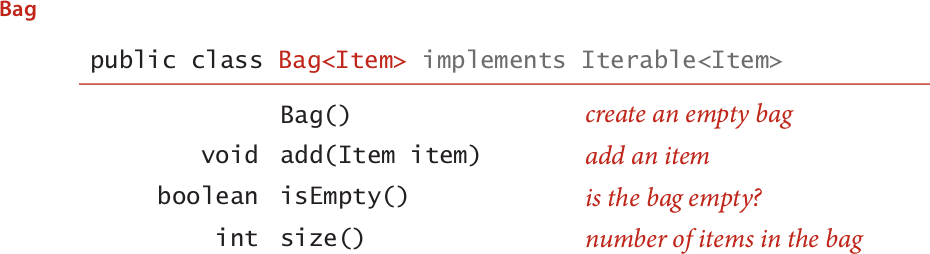
\includegraphics[width=0.8\textwidth]{Pics/API-Bag}

\vspace{0.5cm}

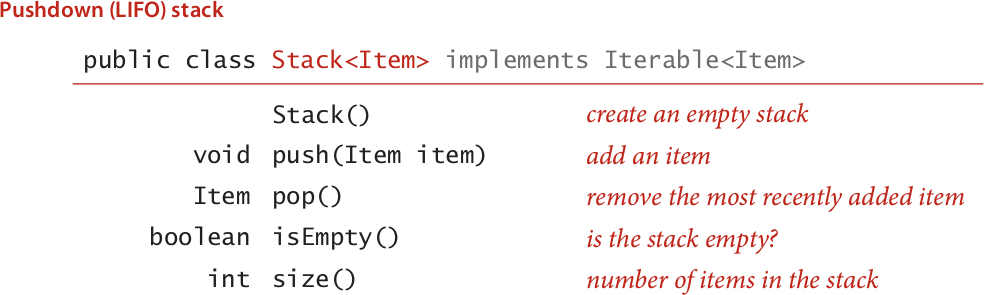
\includegraphics[width=0.8\textwidth]{Pics/API-Stack}

\vspace{0.5cm}

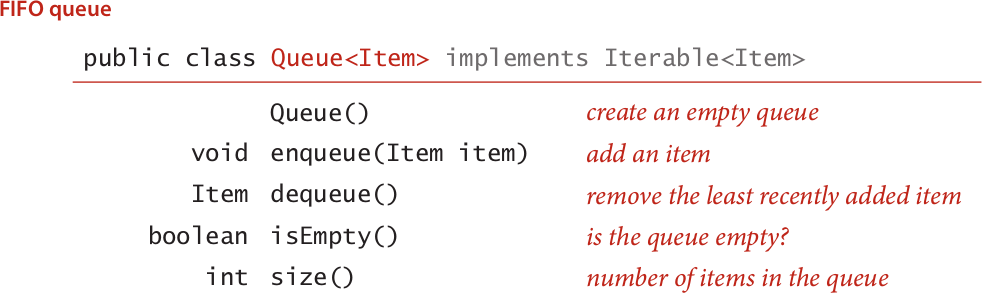
\includegraphics[width=0.8\textwidth]{Pics/API-Queue}

\vspace{0.5cm}

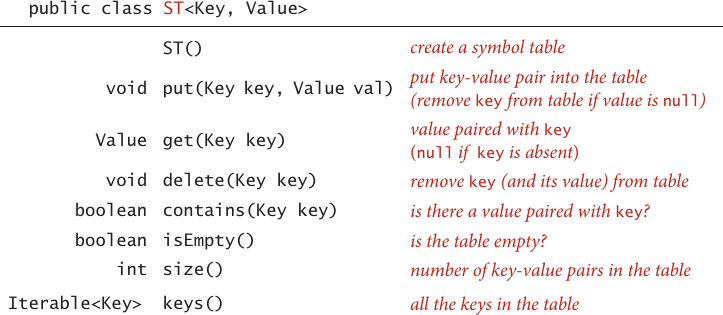
\includegraphics[width=0.8\textwidth]{Pics/API-ST}

\vspace{1cm}

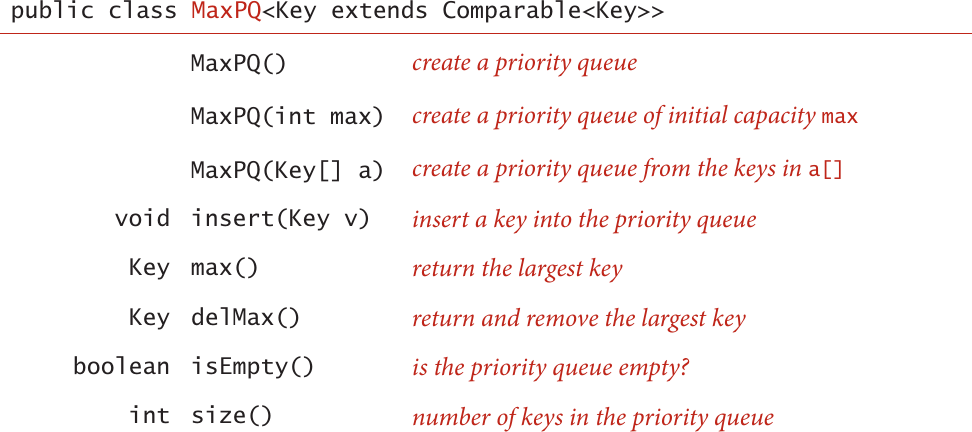
\includegraphics[width=0.8\textwidth]{Pics/API-MaxPQ}

\vspace{1cm}

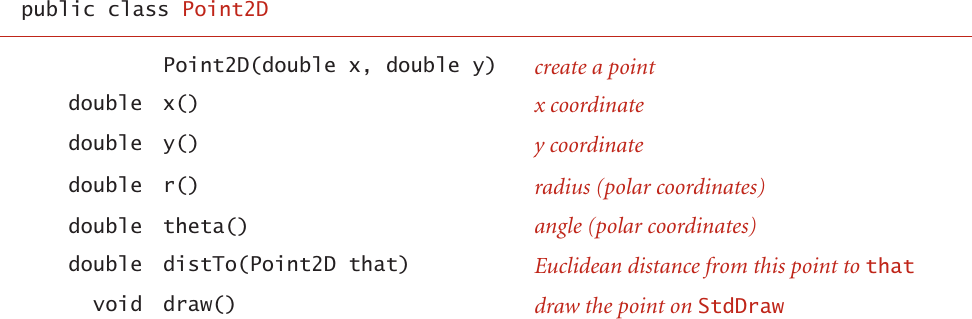
\includegraphics[width=0.8\textwidth]{Pics/API-Point2d}

\vspace{1cm}
\footnote{Í algs4 safninu inniheldur Digraph klasinn \texttt{reverse} aðferð. Sú aðferð er ekki gefin hér. // The Digraph class of the algs4 library contains a \texttt{reverse} method. This method is not supplied here.}
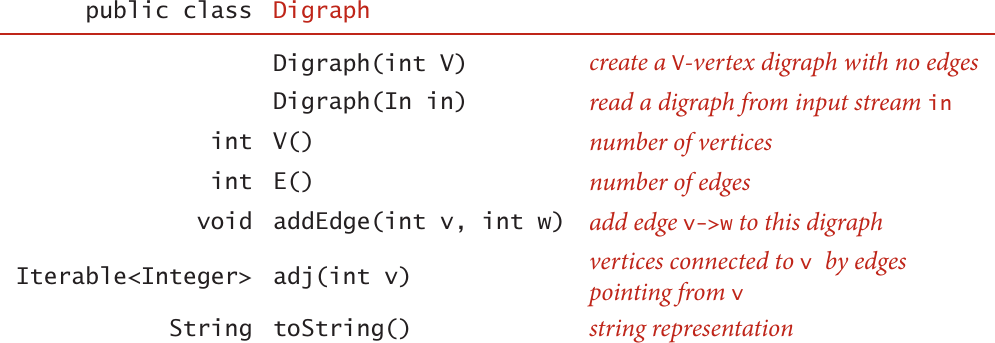
\includegraphics[width=0.8\textwidth]{Pics/API-Digraph}

% 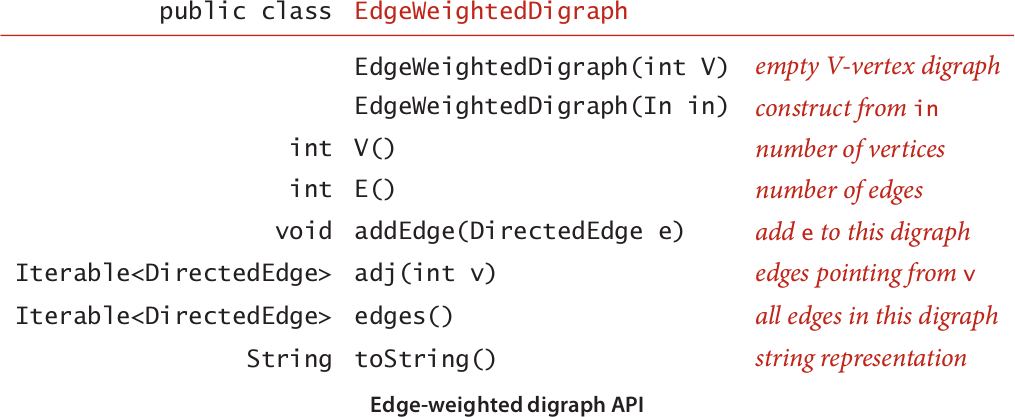
\includegraphics[width=0.8\textwidth]{Pics/API-EWDG}

% \vspace{1cm}

% 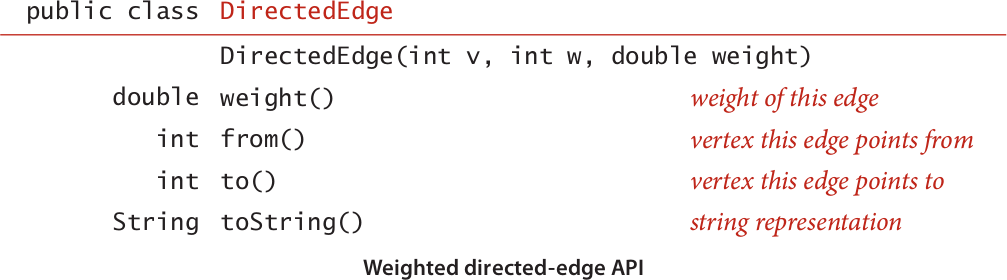
\includegraphics[width=0.8\textwidth]{Pics/API-DE}

% \vspace{1cm}

% 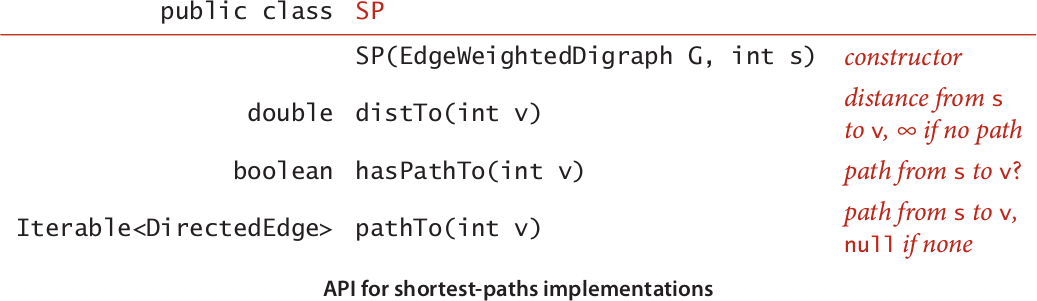
\includegraphics[width=0.8\textwidth]{Pics/API-SP}
\end{center}


\end{questions}
\end{document}